\part{Análisis de requerimientos}\label{part:analisis}
\section{Requerimientos}
\subsection{Funcionales}
\begin{itemize}
	\item La aplicación de PC deberá ser capaz de poder iniciar una conexión segura con el sistema utilizando la misma para enviar los mensajes que el cliente desee.
	\item La aplicación podrá enviar peticiones de forma de obtener el mensaje actual del cartel o incluso establecer uno nuevo. Por otra parte, también podrá pedir los datos de la red a la que el sistema estará conectado o cambiarlos.
	\item La aplicación deberá ser capaz de modificar parámetros de animación tales como frecuencia de parpadeo y velocidad de desplazamiento lateral o estaticidad.
	\item La aplicación permitirá al usuario, ingresar por teclado el mensaje que desea mostrar mediante los caracteres que se establecen en el estándar de codificación de caracteres ISO/IEC 8859-1 (ver \cite{CodifChar}).
	\item El cartel deberá poder procesar sólo mensajes a través del protocolo diseñado específicamente para este proyecto (ver sección \ref{sec:protocolo})
	\item El cartel deberá mostrar los mensajes que desee el usuario de forma legible.
	\item El cartel deberá poder almacenar y modificar sus credenciales de red de forma de poder conectarse al WiFi que el cliente desee.
	\item El cartel deberá mantener los datos de configuración y del mensaje que muestra, aún cuando el mismo haya sido desconectado de la red inalámbrica o de la red eléctrica.
\end{itemize}

\subsection{No funcionales}
\begin{itemize}
	\item El tiempo de respuesta del cartel no debe exceder los cinco segundos.
	\item El sistema entero no debe consumir mas de 30 Watts bajo operación normal.
	\item El sistema deberá ser capaz de aceptar sólo conexiones por TLS \cite{TLS} de forma que las conexiones y el intercambio de paquetes sea cifrado y seguro.
\end{itemize}

\subsection{Interacción con el usuario}
	
	Se denomina usuario del sistema a toda persona con acceso autorizado a su configuración y puesta en marcha.	El usuario tendrá la posibilidad de agregar o quitar módulos esclavos al cartel con el fin de proveerle mayor longitud, de acceder al panel de configuración del cartel para modificar su mensaje y características del mismo.
	
	Para operar correctamente el cartel, únicamente es necesario que el usuario tenga a su disposición una PC, en la cual utilizará un aplicativo desarrollado con una interfaz gráfica para controlar el cartel. Para realizar la instalación del sistema, se requiere solamente al manual de instalación (ver \ref{sec:inst-hw}).

	No es necesario que el usuario tenga conocimientos de programación.
	Sin embargo, una noción básica de electrónica es deseable para evitar que algún componente o conexión eléctrica del sistema se vea perjudicada durante su instalación.

\section{Especificaciones físicas}

	El sistema está conformado por módulos de dos tipos claramente distinguibles.

	El módulo maestro, que se caracteriza por tener la ficha de alimentación y no estar conectada a una matriz de LEDs, se encarga de controlar la cadena de módulos esclavos. Sólo un módulo de este tipo es necesario por cartel.

	Por otro lado, están los módulos esclavos, que se encargan de controlar su matriz de LEDs para representar un mapa de bits y de funcionar como eslabón en la cadena de módulos esclavos. Se puede ver en la figura \ref{fig:dibujo-real} un dibujo ilustrativo exhibiendo los componentes más relevantes del sistema.
	\begin{description}
		\item[A: ] Fuente de alimentación (AC 220V a 5V DC).
		\item[B: ] Cables de interconexión maestro-esclavo y esclavo-esclavo.
		\item[C: ] Módulo esclavo.
		\item[D: ] Módulo maestro.
		\item[E: ] Cables de conexión a la matriz de LEDs.
		\item[F: ] Matriz de LEDs.
		\item[G: ] Pulsador de reset.
		\item[H: ] Jumpers de configuración.
		\item[I: ] NodeMCU ESP-12
		\item[J: ] MAX7219.
	\end{description}
	
	\begin{figure}[ht!]
		\begin{center}
			\centering
			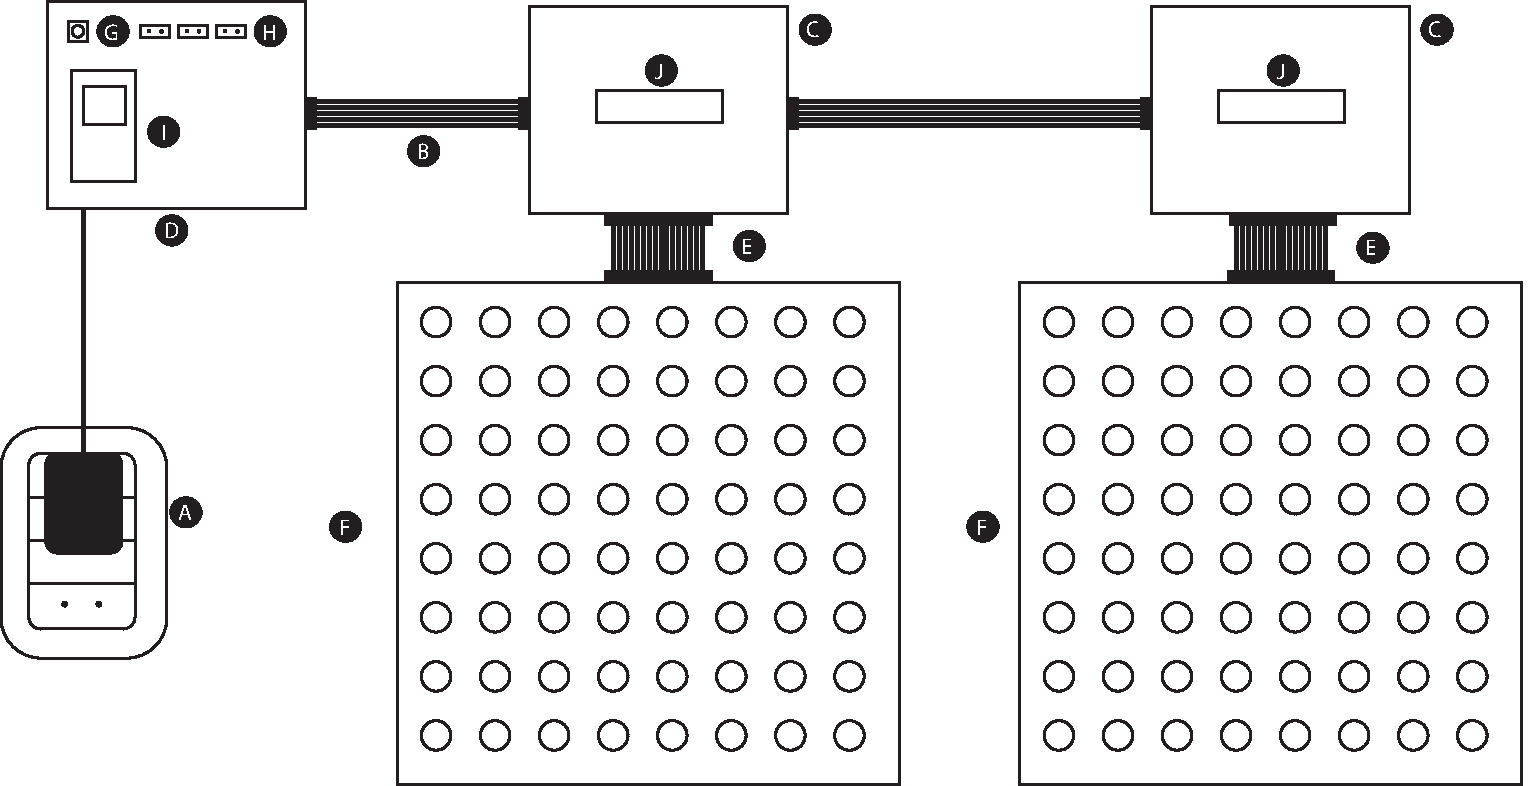
\includegraphics[width=\linewidth]{imagenes/dibujo-fisico.pdf}
			\caption{Dibujo ilustrativo del hardware del sistema.}
			\label{fig:dibujo-real}
		\end{center}
	\end{figure}
